\documentclass[runningheads]{llncs}
\usepackage[T1]{fontenc}
\usepackage[utf8]{inputenc}
\usepackage{lmodern}
\usepackage{amsmath,amssymb}
\usepackage{graphicx,booktabs,tabularx,longtable,array,ragged2e}
\usepackage{float,placeins}
\usepackage{cite}
\usepackage{xurl}
\usepackage[hidelinks]{hyperref}
\usepackage{microtype}
\newcolumntype{Y}{>{\RaggedRight\arraybackslash}X}
\newcolumntype{P}[1]{>{\RaggedRight\arraybackslash}p{#1}}
\setlength{\parindent}{0pt}
\setlength{\parskip}{4pt}
\setlength{\tabcolsep}{2.5pt}
\renewcommand{\arraystretch}{1.16}
\title{Forecasting and Grouping Indian States for Cyber-Police Planning, 2018--2022}
\titlerunning{Forecasting and Grouping Indian States for Cyber-Police Planning}
\author{Abhirup Chakraborty\inst{1}}
\authorrunning{A. Chakraborty}
\institute{Department of Computer Science, Ramanujan College, University of Delhi, New Delhi, India}
\begin{document}
\raggedbottom
\maketitle
\begin{abstract}
State-level cyber-crime registrations in India rose sharply between 2018 and 2022, but five annual observations limit forecast reliability. Using NCRB data for 36 States/UTs (35 modelled), we compare persistence, State means, pooled ordinary least squares, linear ridge and quadratic ridge using a 2022 holdout and three rolling origins with origin-specific tuning. Persistence has the lowest mean RMSE (999.9 \ensuremath{\pm} 417.6 registrations) and a persistence-relative MAE of 1.00; its pooled training-scaled MASE is 1.00 \ensuremath{\pm} 0.47. Linear ridge improves median absolute error for the ten largest States by 2021 volume (394 versus 877), although its 2022 overall RMSE is higher. Excluding Telangana, ridge RMSE is 816 versus 1,082 for persistence. National registrations correlate with internet subscribers (r = 0.981) and UPI volume (r = 0.987) on log scales. A conditional tele-density ablation provides little improvement (ridge RMSE 1,833 versus 1,855); the 2022 cross-section correlation is \ensuremath{-}0.03. K-means and Ward clustering support a descriptive four-tier planning scheme, although silhouette scores favour two groups. Persistence is therefore a useful default benchmark, with ridge and service tiers as supplementary planning tools. Registrations measure recorded workload, not true incidence.
\keywords{Cyber-crime \and NCRB \and Forecasting \and Ridge regression \and Clustering \and Tele-density \and UPI}
\end{abstract}

\FloatBarrier
\section{Introduction}
National cyber-crime registrations rose from 27,248 in 2018 to 65,893 in 2022 \cite{ref1,ref2}, equivalent to a compound annual growth rate of 24.7\%. For cyber-police planning, the question is how much recorded workload to anticipate and which States have similar historical profiles. This note asks whether simple trend forecasts beat persistence, whether digital penetration is associated with registrations, and whether descriptive service tiers offer a useful planning framework. These questions relate to SDG 9 and SDG 16.

\FloatBarrier
\section{Related work}
Recorded crime is an incomplete measure of victimisation: the distinction between actual and recorded events is well established \cite{ref3,ref4}, and the UNODC cybercrime study highlights measurement difficulties \cite{ref5}. Cyber-criminology and work on online victimisation provide context for interpreting these counts \cite{ref6,ref7}. Rosenfeld and Berg demonstrate the importance of data preparation and validation in forecasting crime rates \cite{ref8}. Cruz-Nájera et al. find that simple techniques can be competitive for short crime series \cite{ref9}, consistent with the importance of benchmarks in the M4 competition \cite{ref10}. Glaser et al. show how fixed-effects panel count models can be evaluated for crime forecasting \cite{ref11}. Hybrid deep-learning and smoothing models have been tested on richer crime histories \cite{ref12}, and Mao et al. examine spatiotemporal count prediction with neural models \cite{ref13}. Wu et al. evaluate additional mobility features for short-term crime prediction \cite{ref14}, while Curtis and Oxburgh describe barriers to cyber-crime reporting \cite{ref15}. Chandra examines India's national cyber-crime reporting portal and its institutional challenges \cite{ref16}. Unlike studies with richer temporal or spatial data, this note focuses on a short annual Indian State panel, compares forecasts with a simple baseline using strictly chronological tuning, and combines error diagnostics with descriptive service tiers.

\FloatBarrier
\section{Data and its limits}
The NCRB file contains 28 States, eight Union Territories and three aggregate rows \cite{ref1,ref2}. Aggregate rows are removed for modelling. Ladakh has no separate values in 2018--2019 and is excluded from the balanced panel; Jammu and Kashmir's earlier boundary definition is a comparability limitation. The 35 remaining entities provide 175 observations, of which 140 are used for the final training window and 35 for the 2022 test. Reported zeros are retained. In 2022, the maximum is 15,297 (Telangana) and the minimum is 1 (Mizoram and Lakshadweep). Figure~\ref{fig:1} shows the skew using log(1 + registrations).

\begin{table}[H]
\centering
\caption{Variables, coverage and missing-data audit.}\label{tab:1}
\small
\begin{tabularx}{\linewidth}{@{}P{.24\textwidth}P{.19\textwidth}P{.23\textwidth}Y@{}}
\toprule
\textbf{Dataset / fields} & \textbf{Rows and years} & \textbf{Unit / source} & \textbf{Missing values} \\
\midrule
NCRB: serial, State/UT, 2018--2022 & 36 entity rows; 2018--22 & Identifier; registrations \cite{ref1,ref2} & Serial, State: 0; 2018: 1; 2019: 1; 2020--22: 0 each \\
TRAI: circle, annual tele-density & 19 circles; 2018--22 & Connections per 100 people \cite{ref17} & 0 in every column \\
Circle mapping: State, circle, note & 36 mapping rows & Labels; study mapping \cite{ref17} & State/circle: 0; note: 17 (optional) \\
National: year, cyber, tele-density, internet, UPI & 5 annual rows; 2018--22 & Counts; per 100; millions; billions of transactions \cite{ref1,ref17,ref18} & 0 in every column \\
Merged model panel: State, year, t, cases, logcases, circle, tele-density & 175 State-years; 2018--22 & Identifiers, time index, counts, log-counts, per 100 & 0 in every column \\
\bottomrule
\end{tabularx}
\end{table}
\begin{figure}[H]
\centering
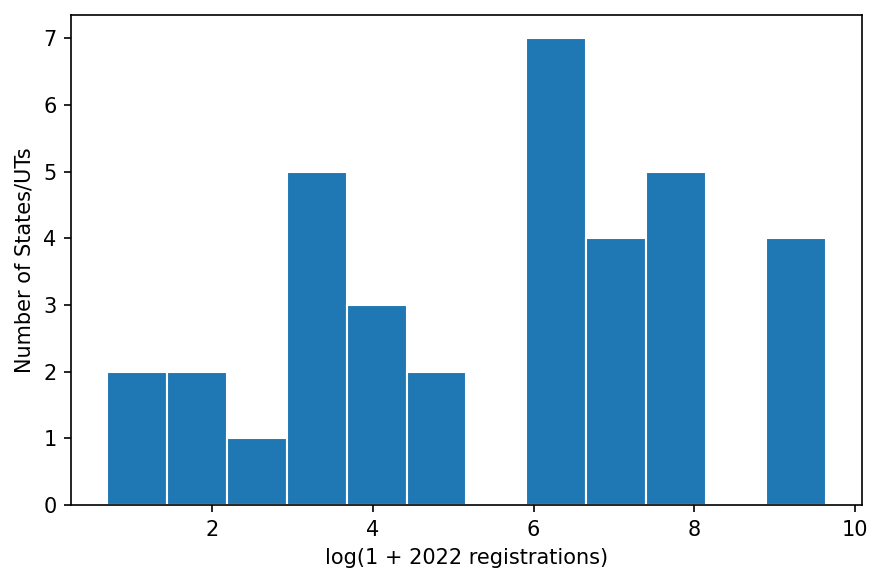
\includegraphics[width=0.67\linewidth,height=0.70\textheight,keepaspectratio]{figures/distribution.png}
\caption{Distribution of 2022 registrations across the 35 modelled entities (log-transformed).}\label{fig:1}
\end{figure}
TRAI year-end indicators provide internet subscriptions and tele-density \cite{ref17}; UPI volumes are financial-year series from NPCI \cite{ref18}, aligned to the calendar-year label rather than exact calendar periods. The 19 service-area tele-density values are mapped to 36 entities, including shared circles and assumed UT mappings (Appendix B). Thus they are proxies, not separately measured State covariates. The full missingness audit is in \path{outputs/missing_data.csv}.

\FloatBarrier
\section{Method and experimental setup}
The final holdout trains on 2018--2021 and tests on 2022. Rolling test years are 2020, 2021 and 2022, each with an expanding training window beginning in 2018. For each ridge model and origin, alpha is selected by minimising count-scale RMSE on the last available training year, using only earlier years to fit the candidate model. The grid is \{0.1, 1, 10, 100, 1000\}; after tuning, the model is refitted on all pre-test data. Validation years are 2019, 2020 and 2021 respectively. Both ridge specifications select 0.1 for 2020 and 2021; for 2022, linear ridge selects 0.1 and quadratic ridge 1.0. In the earliest inner fit, only 2018 is available, so trend coefficients cannot be validated and selection reflects State-effect shrinkage. Two distinct years cannot identify curvature independently; regularisation permits a quadratic forecast but its 2020 result is exploratory. A common-origin sensitivity table (2021--2022) is supplied in \path{outputs/backtest_common_origins.csv}.

Persistence predicts the previous count; the State-mean baseline uses the mean of all pre-test counts. Pooled OLS estimates one common trend with State indicators. Let $y_{st}$ denote registrations for State s in year t, $z_{st}=\ln(1+y_{st})$, $\mathbf{x}_s$ the one-hot State vector and t the year minus 2018. The ridge specification \cite{ref19} is:

\begin{align*}
\hat z_{st} &= b_0+\mathbf{x}_s^{\mathsf T}\mathbf a+\beta_1t
  \quad (+\beta_2t^2\text{ in quadratic ridge}),\\
\text{Minimise}\quad &\sum_{s,t}(z_{st}-\hat z_{st})^2
 +\alpha\left(\lVert\mathbf a\rVert^2+\sum_j\beta_j^2\right),\\
\hat y_{st} &= \exp\bigl(\max(0,\hat z_{st})\bigr)-1.
\end{align*}
The intercept $b_0$ is not penalised. Models are fitted on log-counts and evaluated on counts without rounding. For an origin with n = 35 entities, $e_s=y_s-\hat y_s$:

\begin{align*}
\mathrm{RMSE}&=\sqrt{\frac{1}{n}\sum_s e_s^2},
&\mathrm{MAE}&=\frac{1}{n}\sum_s|e_s|,\\
R^2&=1-\frac{\sum_s e_s^2}{\sum_s(y_s-\bar y)^2},\\
\text{Relative MAE}&=\frac{\mathrm{MAE}(\text{model})}{\mathrm{MAE}(\text{persistence})},\\
\text{Pooled MASE}&=\frac{\mathrm{MAE}(\text{model})}{\frac{1}{n(T-1)}\sum_s\sum_{t=2}^{T}|y_{st}-y_{s,t-1}|}.
\end{align*}
Relative MAE uses the same test year; $T$ is the number of training years.
The training-scaled measure adapts MASE \cite{ref20} to a pooled panel by using a common training denominator rather than averaging State-specific ratios (some States have zero training differences). The original report's ``MASE'' was relative MAE; it is now explicitly labelled. Persistence always has relative MAE 1.00, but not necessarily pooled MASE 1.00. Fold means and sample standard deviations use three origins; these are descriptive spreads, not confidence intervals \cite{ref21}.

The tele-density specification adds $\gamma D_{st}$ (or $\gamma\ln D_{st}$) to the log model, with the linear ridge alpha held at the trend-only choice. Observed 2022 D is used, making this a conditional holdout ablation rather than a real-time forecast. Clustering uses five-year log-count vectors standardised by year, k-means (20 restarts) \cite{ref22}, Ward linkage \cite{ref23} and silhouette scores \cite{ref24} for k = 2--6. Four groups are retained for operational granularity. The random seed is 42; implementations use scikit-learn \cite{ref25}.

\FloatBarrier
\section{Forecasting results}
\begin{table}[H]
\centering
\caption{2022 holdout and rolling-origin mean $\pm$ sample SD (revised original Table 1).}\label{tab:2}
\scriptsize
\begin{tabularx}{\linewidth}{@{}P{.16\textwidth}P{.11\textwidth}P{.10\textwidth}P{.075\textwidth}YYY@{}}
\toprule
\textbf{Model} & \textbf{2022 RMSE} & \textbf{2022 MAE} & \textbf{2022 R\ensuremath{^2}} & \textbf{RMSE mean / SD} & \textbf{Rel. MAE / SD} & \textbf{MASE / SD} \\
\midrule
Persistence & 1,359.8 & 580.8 & 0.861 & 999.9 \ensuremath{\pm}\allowbreak 417.6 & 1.00 \ensuremath{\pm}\allowbreak 0.00 & 1.00 \ensuremath{\pm}\allowbreak 0.47 \\
State mean & 1,994.0 & 730.0 & 0.702 & 1,388.2 \ensuremath{\pm}\allowbreak 588.8 & 1.33 \ensuremath{\pm}\allowbreak 0.17 & 1.28 \ensuremath{\pm}\allowbreak 0.53 \\
Pooled OLS & 1,909.6 & 717.8 & 0.727 & 1,497.4 \ensuremath{\pm}\allowbreak 710.0 & 1.44 \ensuremath{\pm}\allowbreak 0.36 & 1.45 \ensuremath{\pm}\allowbreak 0.72 \\
Ridge & 1,854.7 & 646.5 & 0.742 & 1,485.6 \ensuremath{\pm}\allowbreak 432.9 & 1.48 \ensuremath{\pm}\allowbreak 0.33 & 1.38 \ensuremath{\pm}\allowbreak 0.41 \\
Quadratic ridge & 2,569.5 & 967.0 & 0.505 & 2,306.8 \ensuremath{\pm}\allowbreak 1,346.1 & 2.25 \ensuremath{\pm}\allowbreak 1.16 & 2.30 \ensuremath{\pm}\allowbreak 1.48 \\
\bottomrule
\end{tabularx}
\end{table}
\begin{table}[H]
\centering
\caption{Per-origin results. Each cell gives RMSE / relative MAE / pooled MASE.}\label{tab:3}
\small
\begin{tabularx}{\linewidth}{@{}P{.22\textwidth}YYY@{}}
\toprule
\textbf{Model} & \textbf{2020} & \textbf{2021} & \textbf{2022} \\
\midrule
Persistence & 542.0 / 1.00 / 0.51 & 1,097.8 / 1.00 / 1.04 & 1,359.8 / 1.00 / 1.46 \\
State mean & 817.9 / 1.52 / 0.78 & 1,352.7 / 1.20 / 1.24 & 1,994.0 / 1.26 / 1.83 \\
Pooled OLS & 677.6 / 1.22 / 0.62 & 1,905.0 / 1.86 / 1.93 & 1,909.6 / 1.24 / 1.80 \\
Ridge & 1,009.2 / 1.77 / 0.90 & 1,592.9 / 1.56 / 1.62 & 1,854.7 / 1.11 / 1.62 \\
Quadratic ridge & 848.7 / 1.49 / 0.76 & 3,502.2 / 3.58 / 3.72 & 2,569.5 / 1.66 / 2.42 \\
\bottomrule
\end{tabularx}
\end{table}
Persistence has the lowest mean RMSE, relative MAE and pooled MASE. The State-mean baseline ranks second by mean RMSE; among learned trend models, ridge ranks first. Quadratic ridge is particularly unstable in 2021. The 2022 holdout is also the last rolling origin, not independent evidence in addition to the backtest. The OLS slope is 0.193 log units per year (about 21\% on the multiplicative scale).

Telangana's actual 2022 registrations were 15,297; persistence predicted 10,303 and ridge 5,409. Excluding Telangana reduces ridge RMSE to 816 versus 1,082 for persistence. For the ten highest-volume States selected using 2021 counts, ridge's median absolute error is 394 versus 877, although its RMSE is higher (3,436 versus 2,519). Across all 35 entities, median absolute errors are 135 for ridge and 64 for persistence. These results distinguish typical errors from exposure to large misses. Figure~\ref{fig:2} displays signed errors; Figure~\ref{fig:3} compares observed and predicted counts.

\begin{figure}[H]
\centering
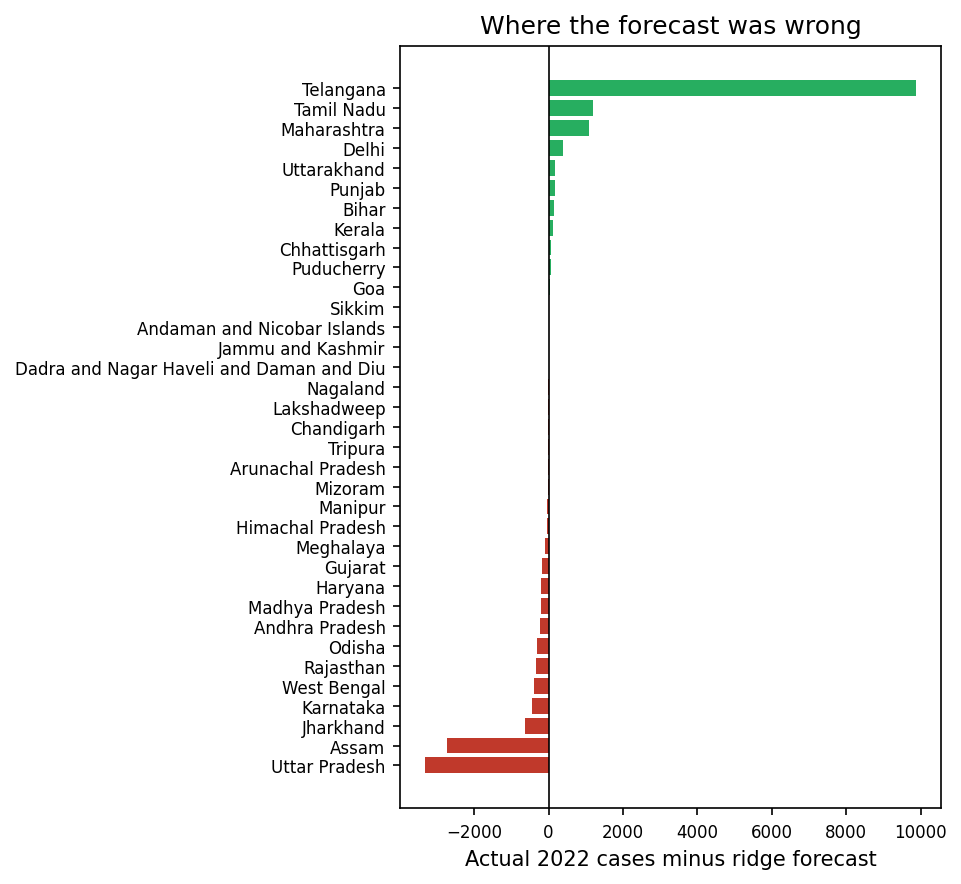
\includegraphics[width=0.76\linewidth,height=0.40\textheight,keepaspectratio]{figures/surprise.png}
\caption{Actual minus ridge forecast for 2022. Positive bars represent underprediction.}\label{fig:2}
\end{figure}
\begin{figure}[H]
\centering
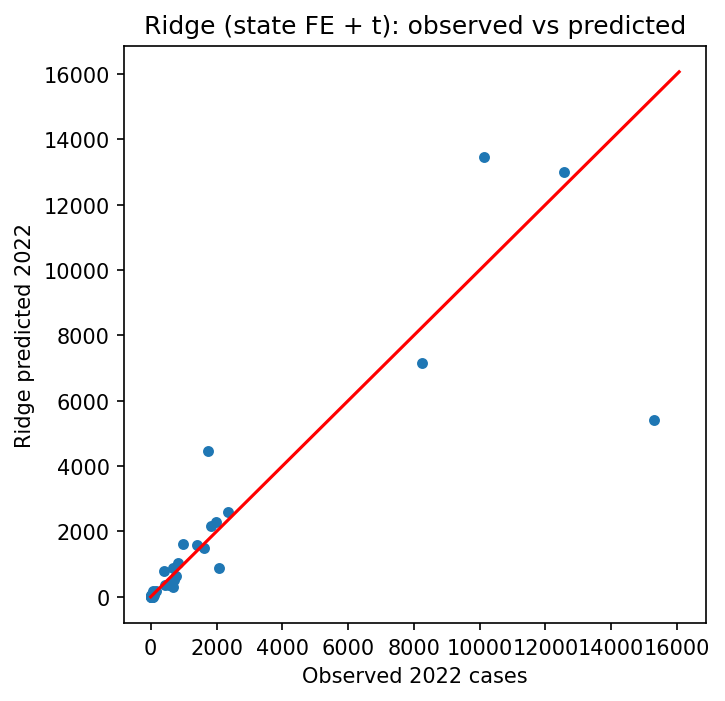
\includegraphics[width=0.76\linewidth,height=0.38\textheight,keepaspectratio]{figures/observed_predicted.png}
\caption{Observed and predicted 2022 registrations; points below the diagonal represent underprediction.}\label{fig:3}
\end{figure}
\FloatBarrier
\section{Digital penetration and service tiers}
The five national log-count observations correlate with log internet subscriptions (r = 0.981) and log UPI volume (r = 0.987). National tele-density falls from 91.45 to 84.56 connections per 100 people and has a negative association with log registrations (r = \ensuremath{-}0.980). These are ecological correlations among trending aggregates, not estimates of individual risk or causal effects. Differences in denominators and time alignment limit interpretation (Fig.~\ref{fig:4}).

\begin{figure}[H]
\centering
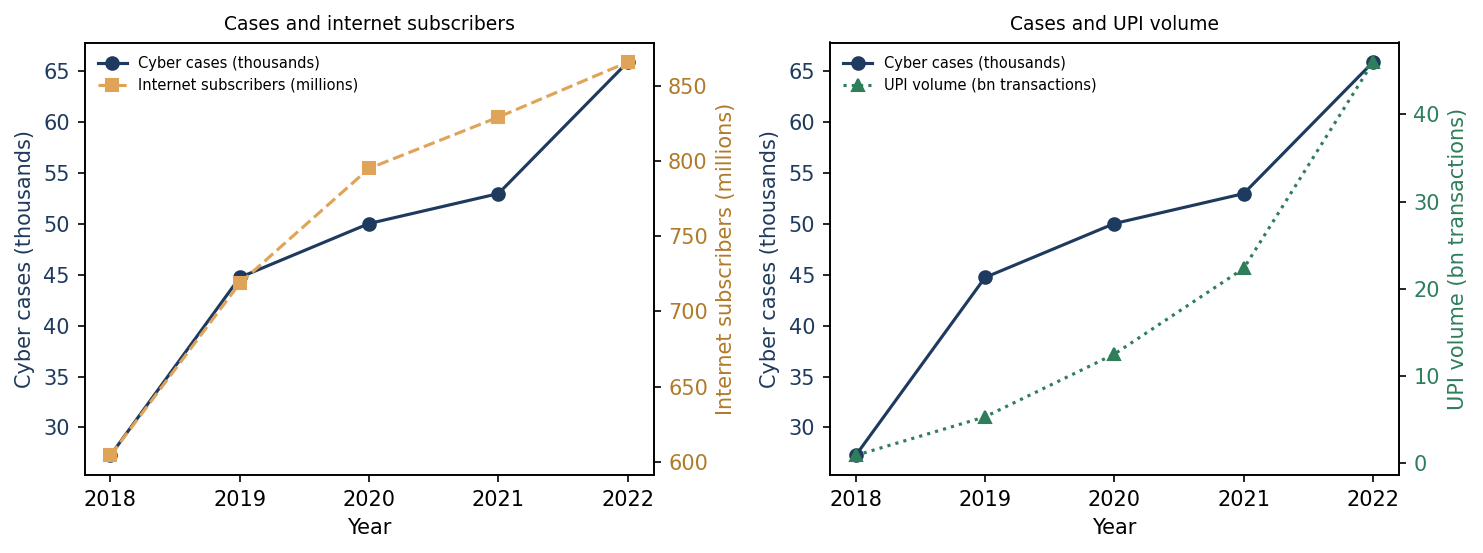
\includegraphics[width=0.97\linewidth,height=0.70\textheight,keepaspectratio]{figures/national_penetration.png}
\caption{All-India cyber-crime registrations, internet subscribers and UPI transaction volumes, 2018--2022.}\label{fig:4}
\end{figure}
\begin{table}[H]
\centering
\caption{Conditional tele-density ablation, 2022 holdout.}\label{tab:4}
\small
\begin{tabularx}{\linewidth}{@{}P{.30\textwidth}rrrY@{}}
\toprule
\textbf{Model} & \textbf{RMSE} & \textbf{MAE} & \textbf{R\ensuremath{^2}} & \textbf{Tele-density coefficient} \\
\midrule
Persistence & 1,359.8 & 580.8 & 0.861 & Not applicable \\
OLS + tele-density & 1,893.1 & 712.4 & 0.731 & -0.0039 \\
OLS + log tele-density & 1,846.2 & 689.1 & 0.745 & -1.3455 \\
Ridge + tele-density & 1,833.0 & 640.4 & 0.748 & -0.0077 \\
\bottomrule
\end{tabularx}
\end{table}
Adding observed 2022 circle tele-density reduces ridge RMSE from 1,855 to 1,833, still above persistence. The OLS coefficient for level tele-density is \ensuremath{-}0.0039 log units per extra connection per 100 people; it is not a causal or statistically tested effect. Pooled, within-State and 2022 cross-sectional correlations are \ensuremath{-}0.118, \ensuremath{-}0.227 and \ensuremath{-}0.025 respectively (Fig.~\ref{fig:5}). The result is a low-power null-style diagnostic, not evidence of absence. Shared circles and limited temporal variation weaken identification.

\begin{figure}[H]
\centering
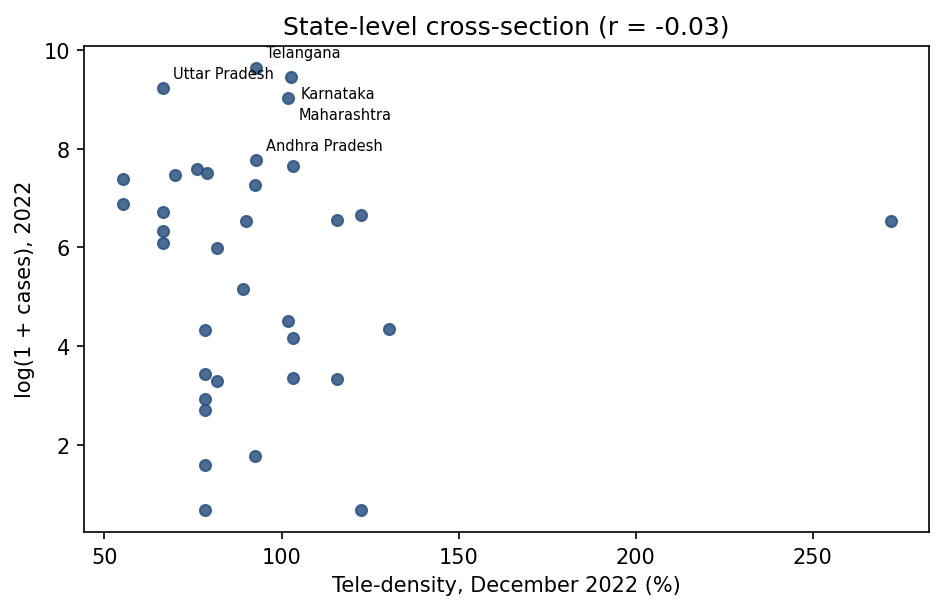
\includegraphics[width=0.76\linewidth,height=0.70\textheight,keepaspectratio]{figures/teledensity.png}
\caption{Circle-level tele-density proxy against 2022 log registrations (r = \ensuremath{-}0.03).}\label{fig:5}
\end{figure}
Silhouette scores favour k = 2 (0.607 for both methods), but four service tiers provide more granular planning categories (k-means 0.432; Ward 0.464). Clusters use the entire 2018--2022 history and therefore describe completed profiles, not future forecasts. Table~\ref{tab:5} lists membership and mean 2022 registrations; Fig.~\ref{fig:6} shows trajectories. The Ward dendrogram and full silhouette comparison appear in Appendix A.

\begin{table}[H]
\centering
\caption{Four descriptive k-means service tiers.}\label{tab:5}
\small
\begin{tabularx}{\linewidth}{@{}P{.075\textwidth}rP{.19\textwidth}Y@{}}
\toprule
\textbf{Tier} & \textbf{n} & \textbf{Mean 2022 registrations} & \textbf{States/UTs} \\
\midrule
C0 & 7 & 18.4 & Mizoram, Nagaland, Sikkim, Andaman and Nicobar Islands, Dadra and Nagar Haveli and Daman and Diu, Lakshadweep, Puducherry \\
C1 & 8 & 63.0 & Arunachal Pradesh, Goa, Himachal Pradesh, Manipur, Meghalaya, Tripura, Chandigarh, Jammu and Kashmir \\
C2 & 12 & 929.0 & Bihar, Chhattisgarh, Gujarat, Haryana, Jharkhand, Kerala, Madhya Pradesh, Punjab, Tamil Nadu, Uttarakhand, West Bengal, Delhi \\
C3 & 8 & 6,763.6 & Andhra Pradesh, Assam, Karnataka, Maharashtra, Odisha, Rajasthan, Telangana, Uttar Pradesh \\
\bottomrule
\end{tabularx}
\end{table}
\begin{figure}[H]
\centering
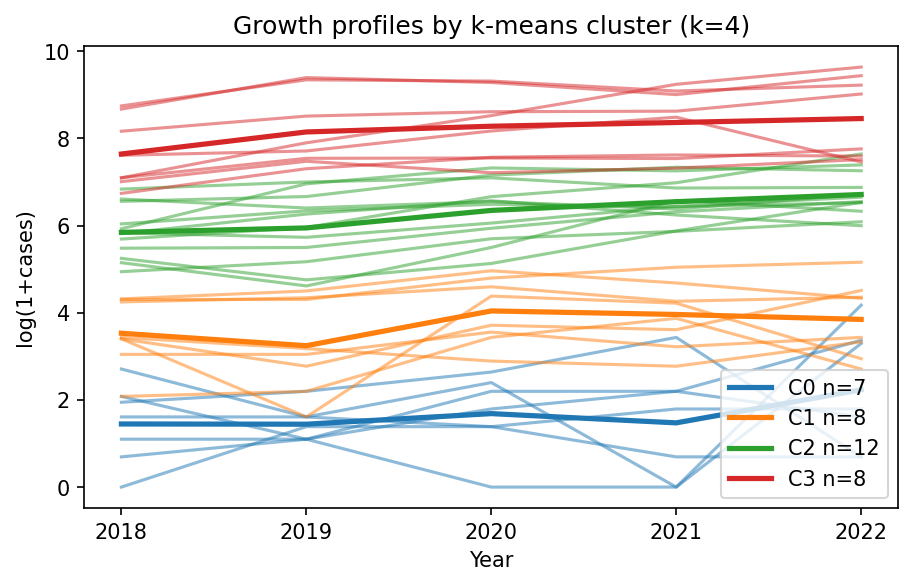
\includegraphics[width=0.97\linewidth,height=0.70\textheight,keepaspectratio]{figures/clusters.png}
\caption{State profiles by k-means tier. Thin lines represent entities; thick lines represent tier means.}\label{fig:6}
\end{figure}
\FloatBarrier
\section{Planning implications and limitations}
Use persistence as a default for State-level recorded workload and report the historical error spread. For high-volume entities, consider ridge alongside persistence and review unusual changes separately. The four tiers offer a way to discuss workload, not a formula for allocating police resources: staffing, investigation complexity, reporting access and local needs also matter. Low registrations may reflect reporting barriers rather than low harm. The panel contains only five annual observations, and the three rolling errors cannot establish reliable prediction intervals. Boundary changes, financial-year alignment, approximate circle mapping, and non-causal correlations further constrain inference. No results rank individual people or State safety.

\FloatBarrier
\section{Conclusion}
With this short panel, persistence outperforms all trend models on average after leakage-free tuning. Ridge remains useful as a complementary estimate for typical high-volume entities, but its aggregate errors are sensitive to Telangana. Tele-density adds little in the conditional comparison. Future work should extend the time series, test lagged State-level indicators and compare forecast intervals, while retaining transparent baseline comparisons.

\FloatBarrier
\section*{Declarations}
Data availability. NCRB data are distributed through OGD India under the Government Open Data Licence (GODL-India) \cite{ref2}. The supplied raw XLS and its XLSX conversion were accessed for revision on 26 November 2026; the original OGD download date is not recorded. The source URL is \url{https://www.data.gov.in/resource/stateut-wise-number-cases-registered-under-cyber-crimes-from-2018-to-2022}. TRAI data are transcribed in \path{data/teledensity_circle.csv}; the circle-to-State mapping is in \path{data/circle_state_map.csv}. National UPI values follow the financial-year series \cite{ref18}.

Code availability. The project repository is \url{https://github.com/abhirupchak/cyber-crime-forecasting-51}. The revised script \path{code/run_experiments.py} regenerates the CSV tables and figures with seed 42; requirements.txt and README.md document the environment. The revised analysis code is available at repository commit \texttt{3f5d62983ef2}.

Generative AI use. ChatGPT (OpenAI) and OpenCode were used to assist with code development, debugging, statistical analysis, interpretation of experimental results, and manuscript preparation and revision. Numerical results are generated from the documented data by the accompanying Python scripts. The author is responsible for reviewing and verifying the methodology, results, references and final manuscript.

\begin{thebibliography}{99}
\bibitem{ref1} National Crime Records Bureau, Crime in India 2022. New Delhi, India: Ministry of Home Affairs, 2023.

\bibitem{ref2} Open Government Data Platform India, ``State/UT-wise number of cases registered under cyber crimes, 2018--2022,'' NCRB. [Online]. Available: \url{https://www.data.gov.in/resource/stateut-wise-number-cases-registered-under-cyber-crimes-from-2018-to-2022}. Supplied dataset accessed Nov. 26, 2026.

\bibitem{ref3} A. D. Biderman and A. J. Reiss, ``On exploring the dark figure of crime,'' Ann. Amer. Acad. Polit. Soc. Sci., vol. 374, no. 1, pp. 1--15, 1967, doi: 10.1177/000271626737400102.

\bibitem{ref4} W. G. Skogan, ``Dimensions of the dark figure of unreported crime,'' Crime Delinq., vol. 23, no. 1, pp. 41--50, 1977, doi: 10.1177/001112877702300104.

\bibitem{ref5} United Nations Office on Drugs and Crime, Comprehensive Study on Cybercrime. Vienna, Austria: UNODC, 2013.

\bibitem{ref6} K. Jaishankar, Ed., Cyber Criminology: Exploring Internet Crimes and Criminal Behavior. Boca Raton, FL, USA: CRC Press, 2011.

\bibitem{ref7} D. Halder and K. Jaishankar, Cyber Crime and the Victimization of Women: Laws, Rights and Regulations. Hershey, PA, USA: IGI Global, 2011.

\bibitem{ref8} R. Rosenfeld and M. Berg, ``Forecasting future crime rates,'' J. Contemp. Criminal Justice, vol. 40, no. 1, 2024, doi: 10.1177/10439862231190215.

\bibitem{ref9} M. A. Cruz-Nájera et al., ``Short time series forecasting: Recommended methods and techniques,'' Symmetry, vol. 14, no. 6, Art. no. 1231, 2022, doi: 10.3390/sym14061231.

\bibitem{ref10} S. Makridakis, E. Spiliotis, and V. Assimakopoulos, ``The M4 competition: 100,000 time series and 61 forecasting methods,'' Int. J. Forecasting, vol. 36, no. 1, pp. 54--74, 2020, doi: 10.1016/j.ijforecast.2019.04.014.

\bibitem{ref11} S. Glaser, R. C. Jung, and K. Schweikert, ``Spatial panel count data: Modeling and forecasting of urban crimes,'' J. Spatial Econometrics, vol. 3, Art. no. 2, 2022, doi: 10.1007/s43071-021-00019-y.

\bibitem{ref12} U. M. Butt, S. Letchmunan, F. H. Hassan, and T. W. Koh, ``Hybrid of deep learning and exponential smoothing for enhancing crime forecasting accuracy,'' PLoS ONE, vol. 17, no. 9, Art. no. e0274172, 2022, doi: 10.1371/journal.pone.0274172.

\bibitem{ref13} L. Mao et al., ``Crime forecasting: A spatio-temporal analysis with deep learning models,'' Int. J. Police Sci. Manage., 2025, doi: 10.1177/14727978251337993.

\bibitem{ref14} J. Wu, S. M. Abrar, N. Awasthi, E. Frias-Martinez, and V. Frias-Martinez, ``Enhancing short-term crime prediction with human mobility flows and deep learning architectures,'' EPJ Data Sci., vol. 11, Art. no. 53, 2022, doi: 10.1140/epjds/s13688-022-00366-2.

\bibitem{ref15} J. Curtis and G. Oxburgh, ``Understanding cybercrime in `real world' policing and law enforcement,'' Police J., 2023, doi: 10.1177/0032258X221107584.

\bibitem{ref16} D. Chandra, ``Examining the contours and challenges of National Cybercrime Reporting Portal in countering digital financial frauds,'' J. Victimology Victim Justice, vol. 8, no. 1, 2025, doi: 10.1177/25166069241306546.

\bibitem{ref17} Telecom Regulatory Authority of India, The Indian Telecom Services Performance Indicators, yearly 2019, 2020, 2021 and quarterly Oct.--Dec. 2022. New Delhi, India: TRAI, 2020--2023.

\bibitem{ref18} National Payments Corporation of India, ``UPI product statistics,'' 2023. [Online]. Available: \url{https://www.npci.org.in/what-we-do/upi/product-statistics}

\bibitem{ref19} A. E. Hoerl and R. W. Kennard, ``Ridge regression: Biased estimation for nonorthogonal problems,'' Technometrics, vol. 12, no. 1, pp. 55--67, 1970, doi: 10.1080/00401706.1970.10488634.

\bibitem{ref20} R. J. Hyndman and A. B. Koehler, ``Another look at measures of forecast accuracy,'' Int. J. Forecasting, vol. 22, no. 4, pp. 679--688, 2006, doi: 10.1016/j.ijforecast.2006.03.001.

\bibitem{ref21} R. J. Hyndman and G. Athanasopoulos, Forecasting: Principles and Practice, 3rd ed. Melbourne, Australia: OTexts, 2021. [Online]. Available: \url{https://otexts.com/fpp3/}

\bibitem{ref22} J. MacQueen, ``Some methods for classification and analysis of multivariate observations,'' in Proc. Fifth Berkeley Symp. Math. Statist. Probab., vol. 1, pp. 281--297, 1967.

\bibitem{ref23} J. H. Ward, Jr., ``Hierarchical grouping to optimize an objective function,'' J. Amer. Statist. Assoc., vol. 58, no. 301, pp. 236--244, 1963, doi: 10.1080/01621459.1963.10500845.

\bibitem{ref24} P. J. Rousseeuw, ``Silhouettes: A graphical aid to the interpretation and validation of cluster analysis,'' J. Comput. Appl. Math., vol. 20, pp. 53--65, 1987, doi: 10.1016/0377-0427(87)90125-7.

\bibitem{ref25} F. Pedregosa et al., ``Scikit-learn: Machine learning in Python,'' J. Mach. Learn. Res., vol. 12, pp. 2825--2830, 2011.
\end{thebibliography}

\FloatBarrier
\appendix
\renewcommand{\thefigure}{\thesection\arabic{figure}}
\renewcommand{\thetable}{\thesection\arabic{table}}
\setcounter{figure}{0}\setcounter{table}{0}
\section{Clustering and forecast diagnostics}\label{app:A}
The full per-State forecasts are in \path{outputs/per_state_forecast.csv}. Table~\ref{tab:A1} and Fig.~\ref{fig:A1} provide the clustering cross-check.

\begin{table}[H]
\centering
\caption{Silhouette by k and k-means inertia.}\label{tab:A1}
\small
\begin{tabular}{@{}rrrr@{}}
\toprule
\textbf{k} & \textbf{K-means silhouette} & \textbf{Ward silhouette} & \textbf{Inertia} \\
\midrule
2 & 0.607 & 0.607 & 45.0 \\
3 & 0.477 & 0.489 & 26.0 \\
4 & 0.432 & 0.464 & 17.1 \\
5 & 0.412 & 0.437 & 12.9 \\
6 & 0.389 & 0.423 & 10.2 \\
\bottomrule
\end{tabular}
\end{table}
\begin{figure}[H]
\centering
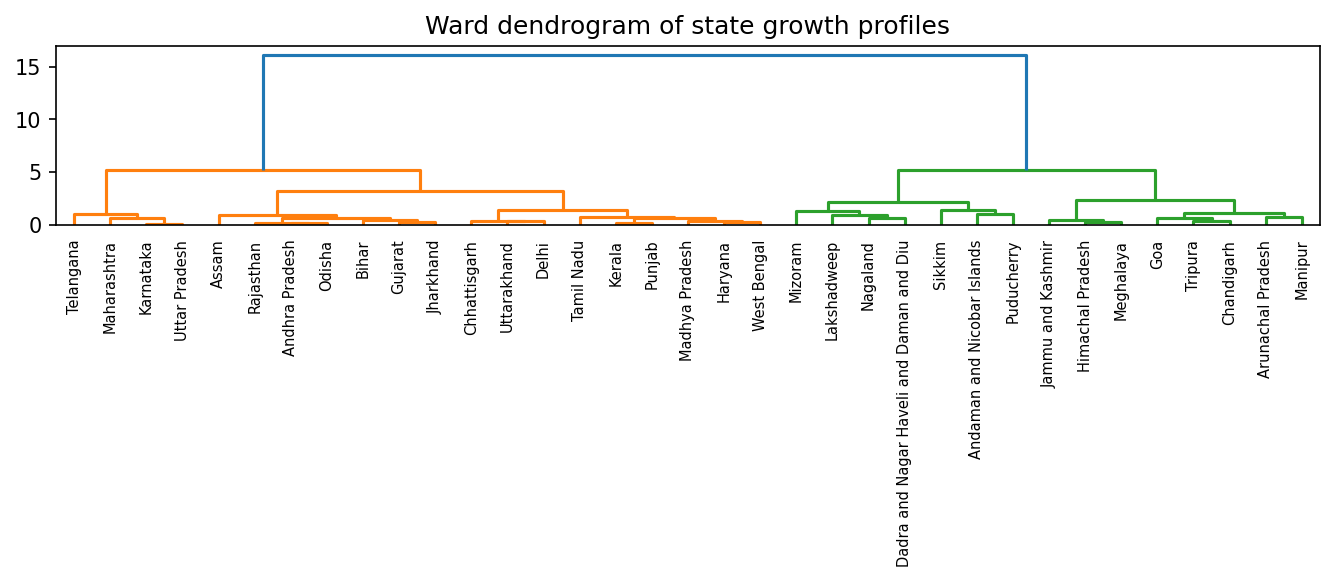
\includegraphics[width=0.97\linewidth,height=0.70\textheight,keepaspectratio]{figures/ward_dendrogram.png}
\caption{Ward dendrogram of the five-year standardised log profiles.}\label{fig:A1}
\end{figure}
\FloatBarrier
\setcounter{table}{0}\setcounter{figure}{0}
\section{Circle-to-State mapping}\label{app:B}
Table~\ref{tab:B1} records the service-area proxy assignment, including assumed mappings.

\small
\begin{longtable}{@{}P{.29\textwidth}P{.25\textwidth}P{.38\textwidth}@{}}
\caption{State/UT, circle and mapping notes.}\label{tab:B1}\\
\toprule
\textbf{State/UT} & \textbf{TRAI circle} & \textbf{Note} \\
\midrule
\endfirsthead
\toprule
\textbf{State/UT} & \textbf{TRAI circle} & \textbf{Note} \\
\midrule
\endhead
\bottomrule
\endfoot
Andhra Pradesh & Andhra Pradesh &  \\
Arunachal Pradesh & North East & NE circle aggregates six states \\
Assam & Assam &  \\
Bihar & Bihar & circle includes Jharkhand \\
Chhattisgarh & Madhya Pradesh & circle includes Chhattisgarh \\
Goa & Maharashtra & circle includes Goa \\
Gujarat & Gujarat &  \\
Haryana & Haryana &  \\
Himachal Pradesh & Himachal Pradesh &  \\
Jharkhand & Bihar & circle includes Jharkhand \\
Karnataka & Karnataka &  \\
Kerala & Kerala &  \\
Madhya Pradesh & Madhya Pradesh &  \\
Maharashtra & Maharashtra &  \\
Manipur & North East & NE circle aggregates six states \\
Meghalaya & North East & NE circle aggregates six states \\
Mizoram & North East & NE circle aggregates six states \\
Nagaland & North East & NE circle aggregates six states \\
Odisha & Orissa &  \\
Punjab & Punjab &  \\
Rajasthan & Rajasthan &  \\
Sikkim & West Bengal & circle includes Sikkim \\
Tamil Nadu & Tamil Nadu &  \\
Telangana & Andhra Pradesh & circle includes Telangana \\
Tripura & North East & NE circle aggregates six states \\
Uttar Pradesh & Uttar Pradesh &  \\
Uttarakhand & Uttar Pradesh & circle includes Uttarakhand \\
West Bengal & West Bengal &  \\
Andaman and Nicobar Islands & Tamil Nadu & assumed TN circle \\
Chandigarh & Punjab & assumed Punjab circle \\
Dadra and Nagar Haveli and Daman and Diu & Gujarat & assumed Gujarat circle \\
Delhi & Delhi &  \\
Jammu and Kashmir & J\&K &  \\
Ladakh & J\&K & circle includes Ladakh \\
Lakshadweep & Kerala & assumed Kerala circle \\
Puducherry & Tamil Nadu & assumed TN circle \\
\end{longtable}
\normalsize

\end{document}
